% !TeX program = xelatex

\PassOptionsToPackage{quiet}{fontspec}
\documentclass[12pt,a4paper,UTF8]{article}
\usepackage{thesis} % 格式控制
\usepackage{indentfirst}
\usepackage{float}
\setlength{\parindent}{2em} % 控制首行缩进  
\addtolength{\parskip}{3pt} % 控制段落距离  
\onehalfspacing % 1.5倍行距  
\graphicspath{{./figures/}} % 指定图片所在文件夹  


\course{机器人学}
\studentname{曹航硕、吴翱臣、康祺}
\studentid{}
\memberone{曹航硕（3240101938）}
\membertwo{吴翱臣（3240106219）}
\memberthree{康祺（3240101043）}
\college{}
\major{}
\instructor{李高峰}
\grade{}
\experimentdate{}
\makepagestyle{}{}




\begin{document}
\maketitlepage % 封面页

\maketoc    %目录页
\section{任务需求}

随着计算机在科研、工程开发和日常学习中的深度普及，高校学生、研究员、开发者等技术人员往往需要长时间保持坐姿并持续面对电脑屏幕。长期低头、前伸颈部或以不对称姿态观察屏幕，容易使颈椎、肩部和背部长期处于非自然受力状态。对于高强度脑力工作场景而言，屏幕位置是否能够匹配用户当前的身体姿态，直接影响工作舒适性、持续工作能力以及长期健康风险。

传统电脑屏幕通常固定摆放在桌面上，或安装在只能由人工调节的机械臂支架上。这类方案虽然能够在初始安装时调整高度、俯仰角和水平位置，但在实际使用过程中并不能主动感知用户姿态变化，也无法根据用户头部朝向和视线方向实时调整屏幕位姿。因此，用户往往需要主动去适应屏幕的位置：当坐姿发生变化、椅背角度改变、身体前后移动，甚至从坐姿切换到站姿时，屏幕与人眼之间的相对位置和朝向都可能偏离合适范围。

本项目的任务需求是设计一套能够根据用户姿态自动调整电脑屏幕位姿的机器人支架系统。系统应通过感知模块获取用户人脸姿态信息，并驱动机械臂式屏幕支架调整末端屏幕的位置与朝向，使屏幕在一定工作空间内尽可能保持正对用户视线并维持合适观看距离。若进一步搭配可自由调节坐姿的人体工学椅，该系统可覆盖用户在大多数坐姿、半躺姿态以及一定站姿场景下的屏幕观看需求，从而减少用户为适应屏幕而产生的不良颈部和躯干姿态。

\begin{figure}[htbp]
    \centering
    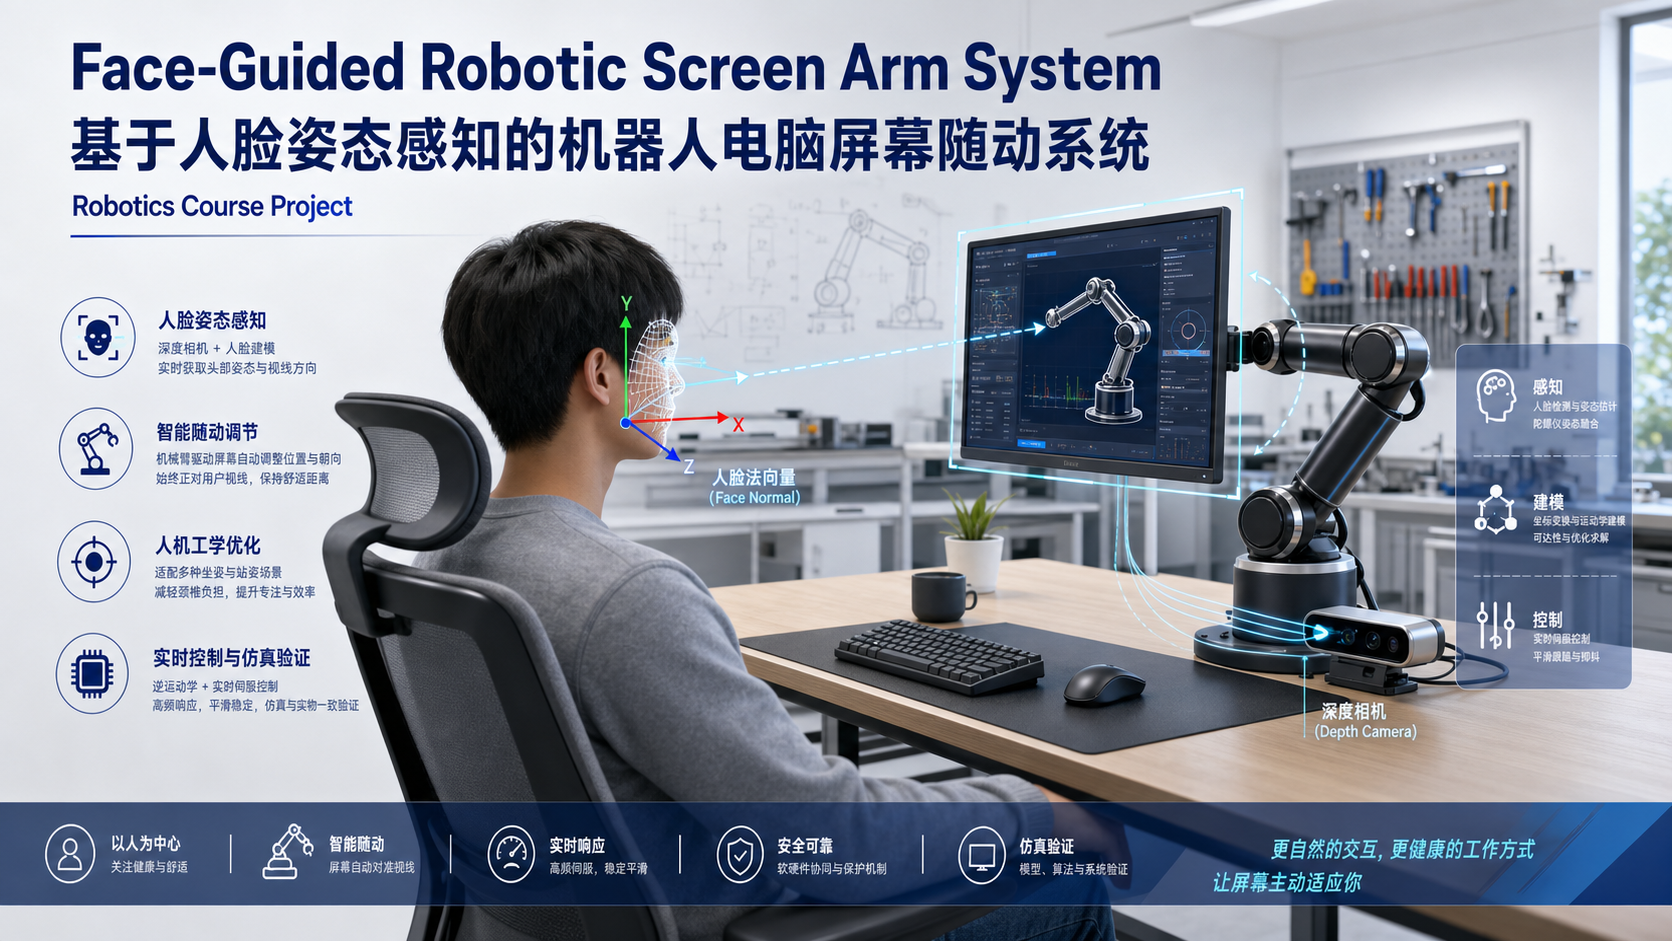
\includegraphics[width=\textwidth]{海报.png}
\end{figure}

\clearpage
\section{总体方案}

本项目的总体思路是将“用户姿态感知”和“机械臂屏幕调节”结合起来，形成一个能够根据人脸朝向自动调整屏幕位姿的桌面机器人系统。系统希望屏幕中心大致位于用户视线方向上，同时让屏幕平面尽量正对用户，从而减少用户主动适应屏幕位置的负担。

系统主要包括人脸姿态建模、坐标变换与目标位姿计算、机械臂运动控制和仿真验证几个部分。深度相机负责获取用户人脸相对于相机坐标系的位姿信息；程序再结合相机在仿真环境中的安装位置和姿态，将该信息转换到世界坐标系中；之后根据人脸方向和合适观看距离计算屏幕目标位姿，并通过逆运动学和轨迹规划指导机械臂运动。

\begin{figure}[htbp]
    \centering
    \begin{tikzpicture}[
        node distance=1.1cm,
        flow/.style={
            rectangle,
            rounded corners=3pt,
            draw=blue!55!black,
            fill=blue!5,
            very thick,
            align=center,
            minimum width=0.72\textwidth,
            minimum height=1.0cm,
            font=\small
        },
        arrow/.style={-{Stealth[length=3mm]}, very thick, draw=blue!60!black}
    ]
        \node[flow] (camera) {深度相机采集用户面部图像\\输出人脸相对相机坐标系位姿 ${}^{C}_{F}T$};
        \node[flow, below=of camera] (transform) {结合相机安装位姿 ${}^{W}_{C}T$\\计算人脸在世界坐标系下的位姿 ${}^{W}_{F}T$};
        \node[flow, below=of transform] (target) {根据人脸方向 ${}^{W}N_F$ 和观看距离 $d$\\计算屏幕末端目标位姿 ${}^{W}_{E}T^{*}$};
        \node[flow, below=of target] (ik) {逆运动学求解\\由 ${}^{W}_{E}T^{*}$ 得到目标关节量 $q^{*}$};
        \node[flow, below=of ik] (traj) {轨迹规划与实时控制\\生成关节运动轨迹 $q(t)$ 并驱动机械臂};
        \node[flow, below=of traj] (screen) {屏幕到达目标位姿 ${}^{W}_{E}T\rightarrow{}^{W}_{E}T^{*}$\\尽量保持正对用户视线};

        \draw[arrow] (camera) -- (transform);
        \draw[arrow] (transform) -- (target);
        \draw[arrow] (target) -- (ik);
        \draw[arrow] (ik) -- (traj);
        \draw[arrow] (traj) -- (screen);
        \draw[arrow] (screen.east) -- ++(0.7,0) |- node[pos=0.25, right, align=center, font=\small] {持续\\更新} (camera.east);
    \end{tikzpicture}
\end{figure}

整体而言，本项目最终形成的是一个“感知--计算--控制--验证”的闭环流程：相机持续感知人脸姿态，程序不断更新屏幕目标位姿，机械臂根据控制算法调整屏幕位置，仿真界面实时展示机械臂、屏幕和用户头部朝向的变化。通过这种方式，可以较直观地验证机器人屏幕支架在不同人脸朝向下的跟随效果。

\clearpage
\section{人脸姿态建模}

在人脸姿态感知部分，本项目采用开源社区中的 3DDFA\_V2（Three-D Dense Face Alignment Version 2）框架作为实时姿态估计方法。该框架的基本流程是：先利用 FaceBoxes 检测图像中的人脸区域，再将人脸图像输入轻量级神经网络，回归三维可变形人脸模型（3D Morphable Model, 3DMM）的参数。通过这些参数，程序可以得到人脸的三维形状、关键点分布以及头部姿态，从而估计人脸相对于相机坐标系的空间朝向。为了便于后续机械臂控制计算，报告中不直接使用完整的人脸网格模型，而是将人脸姿态简化表示为一个从面部中心引出的方向向量。

具体来说，设人脸中心点为 $O_F$，人脸朝向用单位向量 $N_F$ 表示。该向量以 $O_F$ 为起点，方向与用户视线方向近似一致，因此可以用来描述用户当前希望观看屏幕的方向。在相机坐标系下，建模模块输出的人脸姿态可记为 ${}^{C}_{F}T$，其中包含人脸中心位置和人脸坐标系朝向；从该位姿中可以得到相机坐标系下的人脸中心 ${}^{C}O_F$ 以及人脸方向 ${}^{C}N_F$。

在后续计算中，程序会将 ${}^{C}O_F$ 和 ${}^{C}N_F$ 传输给机械臂的计算单元，并结合相机安装位姿 ${}^{W}_{C}T$ 将其转换到世界坐标系下。这样，机械臂控制部分就可以根据世界坐标系中的人脸方向 ${}^{W}N_F$ 和期望观看距离 $d$，计算屏幕末端的目标位姿 ${}^{W}_{E}T^{*}$。这种表示方式虽然没有保留人脸表面的全部几何细节，但足以表达本项目最关心的“用户正在看向哪里”这一姿态信息。

\begin{figure}[htbp]
    \centering
    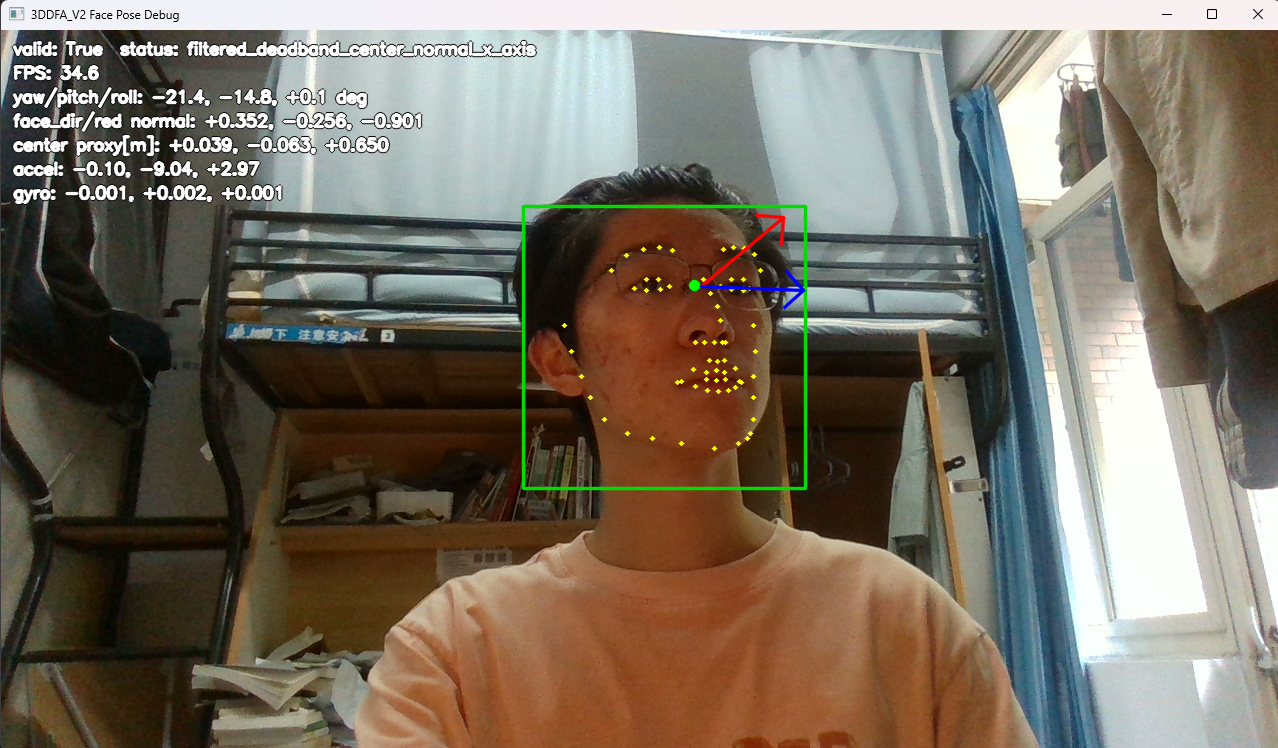
\includegraphics[width=0.88\textwidth]{人脸姿态建模.png}
    \par\vspace{0.3em}
    {\small 红色箭头方向作为用户视线方向}
\end{figure}

\clearpage
\section{机械结构设计}

根据前述任务需求，机械结构需要同时完成屏幕中心位置调整和屏幕朝向调整。为此，本项目设计了一个 6 自由度机器人屏幕支架，其中包含 5 个转动关节和 1 个伸缩关节。整体结构由桌面固定基座、主支撑臂、伸缩臂、屏幕末端支架和深度相机安装位组成，屏幕中心点作为后续控制中的末端参考点。

在自由度分配上，前四个关节主要用于调整末端位置，使屏幕中心能够移动到用户视线方向附近的合适区域；末端两个关节主要用于调整末端姿态，使屏幕平面尽量正对用户人脸。这样的结构划分比较直观，也便于在后续运动学建模中分别理解位置调整和姿态调整的作用。

本项目中的机械臂基座固定在桌面上，深度相机固定安装在基座附近，用于采集用户人脸姿态信息。伸缩关节用于扩大前后方向的工作范围，并辅助调节屏幕与用户之间的观看距离。当前机械结构模型主要服务于仿真验证，结构尺寸和关节范围按照桌面使用场景进行了初步设定。

\begin{table}[htbp]
    \centering
    \small
    \renewcommand{\arraystretch}{1.35}
    \begin{tabular}{@{}c c c c p{0.31\textwidth}@{}}
        \toprule
        关节名称 & 关节类型 & 关节变量符号 & 关节变量取值范围 & 主要职责 \\
        \midrule
        关节 1 & 转动关节 & $\theta_1$ & $[-150^\circ,\,150^\circ]$ & 主要用于调整末端位置。 \\
        关节 2 & 转动关节 & $\theta_2$ & $[-200^\circ,\,20^\circ]$ & 主要用于调整末端位置。 \\
        关节 3 & 转动关节 & $\theta_3$ & $[-170^\circ,\,170^\circ]$ & 主要用于调整末端位置。 \\
        关节 4 & 平动关节 & $d_4$ & $[0,\,0.28]\,\mathrm{m}$ & 主要用于调整末端位置。 \\
        关节 5 & 转动关节 & $\theta_5$ & $[-100^\circ,\,100^\circ]$ & 主要用于调整末端姿态。 \\
        关节 6 & 转动关节 & $\theta_6$ & $[-60^\circ,\,60^\circ]$ & 主要用于调整末端姿态。 \\
        \bottomrule
    \end{tabular}
\end{table}

\begin{figure}[htbp]
    \centering
    \begin{minipage}[t]{0.495\textwidth}
        \centering
        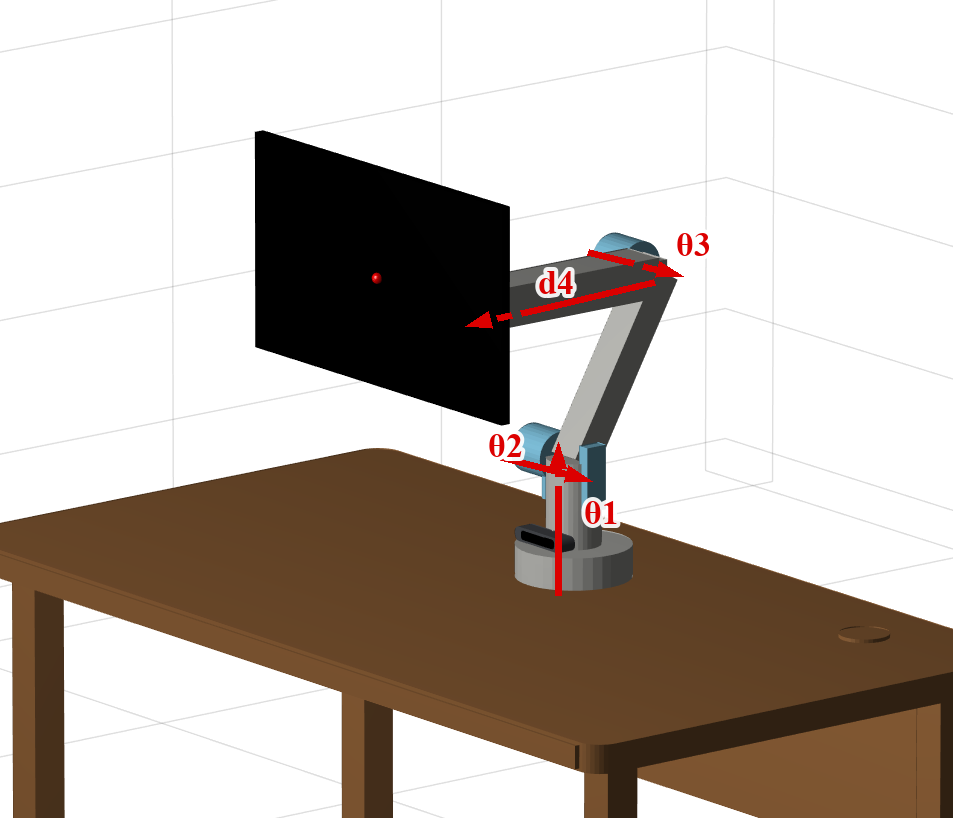
\includegraphics[width=\linewidth]{机械结构1.png}
    \end{minipage}\hfill
    \begin{minipage}[t]{0.495\textwidth}
        \centering
        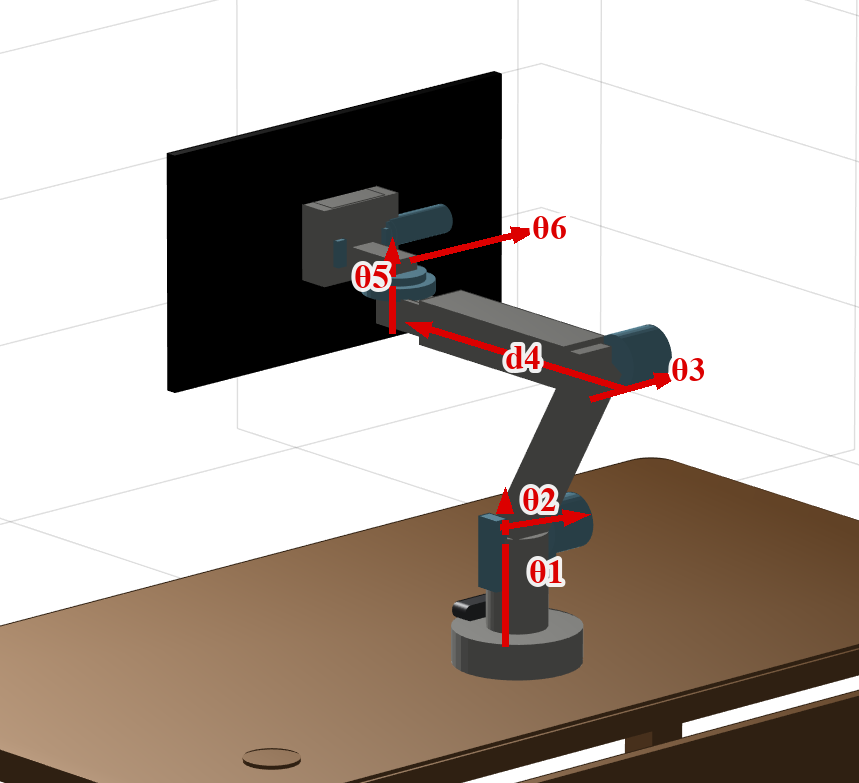
\includegraphics[width=\linewidth]{机械结构2.png}
    \end{minipage}
    \caption{机械臂建模展示}
\end{figure}

\clearpage
\section{运动学建模}

\subsection{坐标系建立}

下面建立机械臂的正运动学模型。该模型中，桌面与机械臂基座之间为固定连接，机械臂本体从基座开始依次经过 6 个运动关节，最后到达屏幕中心点。为了和前文仿真坐标保持一致，世界坐标系记为 $\{W\}$，机械臂基座坐标系记为 $\{0\}$。其中 $\{0\}$ 的原点取在机械臂基座原点处，三个坐标轴方向与世界坐标系相同。

对每个运动关节建立联体坐标系，并使对应坐标系的 $z$ 轴与该关节轴线重合；$x$ 轴沿相邻关节轴线的公法线方向或连杆主要延伸方向选取，$y$ 轴由右手定则确定。由于仿真模型中关节 2、关节 3、关节 4 和关节 6 的轴线并不都与初始坐标系的 $z$ 轴平行，因此在建立 D-H 参量时，需要通过 $\alpha_{i-1}$ 描述相邻关节轴线之间的夹角。

令关节变量为
\[
q=\begin{bmatrix}
\theta_1 & \theta_2 & \theta_3 & d_4 & \theta_5 & \theta_6
\end{bmatrix}^{T}.
\]
根据机械臂的连接方式和各关节轴线方向，可以得到改进 D-H 运动学参量表，如下所示。

\subsection{D-H 运动学参量}

\begin{center}
    \centering
    \normalsize
    \renewcommand{\arraystretch}{1.45}
    \begin{tabular*}{0.66\textwidth}{@{\extracolsep{\fill}}|c|c|c|c|c|}
        \hline
        $i$ & $\alpha_{i-1}$ & $a_{i-1}$ & $d_i$ & $\theta_i$ \\
        \hline
        1 & $0$ & $0$ & $l_1$ & $\theta_1$ \\
        \hline
        2 & $-\pi/2$ & $0$ & $0$ & $\theta_2$ \\
        \hline
        3 & $0$ & $l_2$ & $0$ & $\theta_3$ \\
        \hline
        4 & $-\pi/2$ & $l_3$ & $d_4$ & $0$ \\
        \hline
        5 & $\pi/2$ & $l_4$ & $l_5$ & $\theta_5$ \\
        \hline
        6 & $-\pi/2$ & $l_6$ & $l_7$ & $\theta_6$ \\
        \hline
        E & $0$ & $l_8$ & $0$ & $0$ \\
        \hline
    \end{tabular*}
\end{center}

其中 $l_1=0.160\,\mathrm{m}$，$l_2=0.280\,\mathrm{m}$，$l_3=0.240\,\mathrm{m}$，
$l_4=0.085\,\mathrm{m}$，$l_5=0.024\,\mathrm{m}$，
$l_6=0.070\,\mathrm{m}$，$l_7=0.042\,\mathrm{m}$，$l_8=0.052\,\mathrm{m}$。
其中 $l_1$ 表示基座原点到关节 1 轴线的竖直高度；$l_2$ 表示关节 2 到关节 3 之间的上臂长度；$l_3$ 表示关节 3 到伸缩关节起点之间的前臂固定段长度；$l_4$ 和 $l_5$ 分别表示伸缩滑块末端到关节 5 的水平安装偏移和竖直安装偏移；$l_6$ 和 $l_7$ 分别表示关节 5 到关节 6 的水平安装偏移和竖直安装偏移；$l_8$ 表示关节 6 到屏幕中心点 $\{E\}$ 的末端偏移。

\subsection{正运动学方程}

对于表中第 $i$ 行参量，坐标系 $\{i\}$ 相对于坐标系 $\{i-1\}$ 的齐次变换矩阵为
\[
{}^{i-1}_{i}T=
\begin{bmatrix}
1 & 0 & 0 & 0\\
0 & \cos\alpha_{i-1} & -\sin\alpha_{i-1} & 0\\
0 & \sin\alpha_{i-1} & \cos\alpha_{i-1} & 0\\
0 & 0 & 0 & 1
\end{bmatrix}
\begin{bmatrix}
1 & 0 & 0 & a_{i-1}\\
0 & 1 & 0 & 0\\
0 & 0 & 1 & 0\\
0 & 0 & 0 & 1
\end{bmatrix}
\begin{bmatrix}
\cos\theta_i & -\sin\theta_i & 0 & 0\\
\sin\theta_i & \cos\theta_i & 0 & 0\\
0 & 0 & 1 & d_i\\
0 & 0 & 0 & 1
\end{bmatrix}.
\]
将运动学参量表逐行代入后，可得屏幕中心末端坐标系 $\{E\}$ 相对于基座坐标系 $\{0\}$ 的齐次变换矩阵为
\[
{}^{0}_{E}T
= {}^{0}_{1}T\,{}^{1}_{2}T\,{}^{2}_{3}T\,{}^{3}_{4}T\,
{}^{4}_{5}T\,{}^{5}_{6}T\,{}^{6}_{E}T.
\]
为了表达末端位置与姿态，将该矩阵写成分块形式：
\[
{}^{0}_{E}T=
\begin{bmatrix}
{}^{0}_{E}R & {}^{0}O_E\\
0\ 0\ 0 & 1
\end{bmatrix}.
\]

\subsection{世界坐标系下的末端位姿}

在仿真世界坐标系中，基座坐标系相对于世界坐标系只有固定平移，没有相对转角。由模型文件可知
\[
{}^{W}_{0}T=
\begin{bmatrix}
1 & 0 & 0 & -0.150\\
0 & 1 & 0 & 0\\
0 & 0 & 1 & 0.740\\
0 & 0 & 0 & 1
\end{bmatrix}.
\]
因此，屏幕中心末端坐标系在世界坐标系下的齐次变换矩阵为
\[
{}^{W}_{E}T={}^{W}_{0}T\,{}^{0}_{E}T.
\]

\clearpage
\section{动力学分析}

\subsection{动力学方程}

在前面的运动学建模中，关节变量 $q$ 描述了机械臂的几何位姿；而动力学分析进一步研究关节力矩、连杆惯量、重力和摩擦等因素对运动的影响。对于本项目的屏幕随动支架，机械臂主要承担屏幕、末端支架和深度相机等部件的重力载荷，同时需要在用户头部姿态变化时完成较平稳的跟随运动。因此动力学分析的重点不是高速运动，而是低速跟随过程中的重力补偿、关节驱动力估算和运动平稳性。

令机械臂各连杆质量分别为 $m_i$，质心在世界坐标系下的位置为 ${}^{W}O_{c_i}$，连杆角速度为 $\omega_i$，质心线速度为 $v_{c_i}$。第 $i$ 个连杆的动能可以写为平动动能和转动动能之和：
\[
K_i=\frac{1}{2}m_i v_{c_i}^{T}v_{c_i}
+\frac{1}{2}\omega_i^{T}I_i\omega_i ,
\]
其中 $I_i$ 为连杆绕质心坐标系表示的转动惯量矩阵。机械臂系统总动能为
\[
K=\sum_{i=1}^{6}K_i
=\frac{1}{2}\dot q^{T}M(q)\dot q ,
\]
其中 $M(q)$ 为关节空间惯量矩阵。设重力加速度向量为 $g$，则系统势能可写为
\[
P=-\sum_{i=1}^{6}m_i g^{T}{}^{W}O_{c_i}.
\]

根据拉格朗日方程，取 $L=K-P$，则第 $i$ 个广义坐标满足
\[
\frac{d}{dt}\left(\frac{\partial L}{\partial \dot q_i}\right)
-\frac{\partial L}{\partial q_i}
=\tau_i .
\]
整理所有关节后，可得到机械臂的一般动力学方程：
\[
M(q)\ddot q+C(q,\dot q)\dot q+G(q)+B\dot q+\tau_f
=\tau+J_E^{T}(q)F_E .
\]
式中，$C(q,\dot q)\dot q$ 表示科氏力和离心力项，$G(q)$ 表示重力项，$B\dot q$ 表示粘性阻尼项，$\tau_f$ 表示库仑摩擦等非线性摩擦项，$J_E(q)$ 为屏幕中心末端的雅可比矩阵，$F_E$ 为末端外力。由于本项目的屏幕末端在正常工作时不与外界发生接触，通常可取 $F_E=0$。对转动关节而言，$\tau_i$ 为关节力矩；对第 4 个平动关节而言，对应分量为沿伸缩方向的驱动力。

\subsection{低速随动工况简化}

本项目中机械臂的运行速度较低，目标是让屏幕跟随人脸方向缓慢调整，而不是进行高速抓取或搬运。因此在初步分析时，可以将主要负载近似为重力项和较小的加减速惯性项。若关节运动比较平稳，则有
\[
\left\|M(q)\ddot q+C(q,\dot q)\dot q\right\|
\ll
\left\|G(q)\right\| ,
\]
此时关节所需力矩可近似写为
\[
\tau \approx G(q)+B\dot q+\tau_f .
\]
这说明机械臂在不同姿态下的持载能力是驱动设计的关键，尤其是前几个主要承担屏幕重量的关节。

\subsection{屏幕静载荷估算}

为了得到更直观的量级估计，取一台 24 寸显示器质量约为 $3.5\,\mathrm{kg}$，并考虑末端支架、连接件等附加质量，将末端等效质量保守取为
\[
m_E=4.0\,\mathrm{kg}.
\]
于是末端重力约为
\[
F_E=m_E g=4.0\times 9.81\approx 39.2\,\mathrm{N}.
\]
在最不利的近似姿态下，可将屏幕重力对关节的影响估算为
\[
\tau_i\approx F_E r_i ,
\]
其中 $r_i$ 为屏幕等效质心到第 $i$ 个关节轴线的垂直力臂。根据前述连杆尺寸，取关节 2 到屏幕中心的等效力臂约为 $0.76\,\mathrm{m}$，关节 3 到屏幕中心的等效力臂约为 $0.48\,\mathrm{m}$，末端姿态关节到屏幕中心的偏置约为 $0.05\,\mathrm{m}$，可得表中的载荷估算。

\begin{center}
    \centering
    \small
    \renewcommand{\arraystretch}{1.35}
    \begin{tabular}{|>{\centering\arraybackslash}p{0.14\textwidth}|>{\centering\arraybackslash}p{0.24\textwidth}|>{\centering\arraybackslash}p{0.26\textwidth}|>{\centering\arraybackslash}p{0.24\textwidth}|}
        \hline
        关节 & 主要受载方式 & 屏幕重力载荷估算 & 分析结论 \\
        \hline
        关节 1 & 绕竖直方向偏摆 & 重力力矩近似为 $0$ & 主要考虑转动惯量和摩擦 \\
        \hline
        关节 2 & 支撑主臂和屏幕 & $39.2\times 0.76\approx 29.8\,\mathrm{N\,m}$ & 载荷最大，是重点承载关节 \\
        \hline
        关节 3 & 支撑前臂和末端 & $39.2\times 0.48\approx 18.8\,\mathrm{N\,m}$ & 载荷较大，需要较高保持力矩 \\
        \hline
        关节 4 & 伸缩方向推拉 & 最大重力等效力约 $39.2\,\mathrm{N}$ & 主要关注轴向推力和自锁 \\
        \hline
        关节 5 & 屏幕姿态调节 & $39.2\times 0.05\approx 2.0\,\mathrm{N\,m}$ & 主要关注姿态精度和平稳性 \\
        \hline
        关节 6 & 屏幕姿态调节 & $39.2\times 0.05\approx 2.0\,\mathrm{N\,m}$ & 主要关注姿态精度和平稳性 \\
        \hline
    \end{tabular}
\end{center}

\subsection{屏幕动载荷估算}

上表主要反映静载荷。对于动载荷，可进一步用等效转动惯量进行近似估算。若屏幕等效质量 $m_E$ 距离某关节轴线的等效力臂为 $r_i$，则该质量对该关节的等效转动惯量可近似为
\[
I_{E,i}\approx m_E r_i^2 .
\]
当关节角加速度为 $\ddot q_i$ 时，由末端屏幕引起的惯性力矩约为
\[
\tau_{i,\mathrm{dyn}}\approx I_{E,i}\ddot q_i .
\]
本项目是低速随动系统，取较保守的关节角加速度 $\ddot q_i=2.0\,\mathrm{rad/s^2}$ 进行估算，则关节 2 的屏幕等效惯性力矩约为
\[
\tau_{2,\mathrm{dyn}}
\approx 4.0\times 0.76^2\times 2.0
\approx 4.6\,\mathrm{N\,m},
\]
关节 3 的屏幕等效惯性力矩约为
\[
\tau_{3,\mathrm{dyn}}
\approx 4.0\times 0.48^2\times 2.0
\approx 1.8\,\mathrm{N\,m}.
\]
对于末端姿态关节，由于等效力臂约为 $0.05\,\mathrm{m}$，其屏幕惯性力矩约为
\[
\tau_{5,\mathrm{dyn}}\approx\tau_{6,\mathrm{dyn}}
\approx 4.0\times 0.05^2\times 2.0
\approx 0.02\,\mathrm{N\,m}.
\]
第 4 个平动关节若取伸缩方向加速度 $a_4=0.5\,\mathrm{m/s^2}$，则由屏幕质量引起的附加惯性力约为
\[
F_{4,\mathrm{dyn}}\approx m_E a_4=2.0\,\mathrm{N}.
\]

\subsection{载荷分析结论}

由上述结果可以看出，在本项目的低速工作条件下，动载荷相对于重力静载荷较小。例如关节 2 的静载荷估算约为 $29.8\,\mathrm{N\,m}$，而屏幕引起的附加惯性力矩约为 $4.6\,\mathrm{N\,m}$。因此驱动选型时仍应以静载荷和保持力矩为主，同时用一定安全系数覆盖动载荷、摩擦和模型误差。

上述估算只考虑屏幕和末端安装件的质量，尚未计入各连杆自重、减速器重量和摩擦。因此实际设计中，关节 2 和关节 3 的需求力矩还会进一步增大。由此可以得到一个直接结论：关节 1 主要改变水平偏摆方向，受重力直接影响较小；关节 2 和关节 3 是整机的主要承载关节；关节 4 需要提供足够的伸缩推拉力；关节 5 和关节 6 主要用于调整屏幕姿态，但仍需克服屏幕偏心安装带来的末端力矩。

为了用于后续驱动选型，可以在仿真中沿典型工作空间采样若干组关节状态，并计算每个关节的最大需求：
\[
\tau_{i,\max}=
\max_t
\left|
\left[
M(q)\ddot q+C(q,\dot q)\dot q+G(q)+B\dot q+\tau_f
\right]_i
\right| .
\]
其中对第 4 个平动关节，$\tau_{4,\max}$ 表示最大轴向驱动力。实际选型时还需要考虑模型误差、摩擦、装配偏差和屏幕质量变化，因此应在理论最大值基础上乘以安全系数。

\clearpage
\section{驱动选型}

\subsection{转动关节驱动}

驱动选型的目标是使每个关节在给定工作空间内都能够稳定承受载荷，并按照控制系统给出的轨迹完成运动。由于本项目机械臂用于桌面屏幕支架，运动速度要求不高，但对静止保持、低速平稳性和姿态稳定性要求较高。因此驱动器选型时应优先考虑额定力矩、减速器背隙、编码器精度、保持制动能力和控制接口等因素。

对于转动关节，可采用“伺服电机加减速器”的驱动形式。电机输出力矩与电枢电流近似成正比：
\[
T_{m,i}=C_{T_i}I_i ,
\]
其中 $T_{m,i}$ 为电机输出力矩，$C_{T_i}$ 为力矩常数，$I_i$ 为电机电流。若第 $i$ 个转动关节采用减速比为 $n_i$、效率为 $\eta_i$ 的减速器，则电机侧力矩和关节侧力矩近似满足
\[
\tau_i \approx \eta_i n_i T_{m,i}.
\]
因此，电机额定力矩和峰值力矩应满足
\[
T_{m,i}^{\mathrm{rated}}
\geq
\frac{k_s \tau_{i,\mathrm{rated}}}{\eta_i n_i},
\qquad
T_{m,i}^{\mathrm{peak}}
\geq
\frac{k_p \tau_{i,\max}}{\eta_i n_i}.
\]
其中 $k_s$ 和 $k_p$ 为安全系数，分别用于额定连续工作和短时峰值动作。关节速度也受到减速比限制，若关节最大角速度为 $\dot q_{i,\max}$，则电机最大转速需要满足
\[
\omega_{m,i}^{\max}\geq n_i\dot q_{i,\max}.
\]

\subsection{平动关节驱动}

第 4 个关节为平动关节，适合采用丝杠、同步带或电动推杆等直线驱动方案。若采用丝杠传动，丝杠导程为 $p_4$，传动效率为 $\eta_4$，则轴向力 $F_4$ 与电机力矩近似满足
\[
T_{m,4}
\geq
\frac{k_s F_{4,\max}p_4}{2\pi \eta_4 n_4}.
\]
该关节主要用于扩大屏幕前后方向的可达范围，因此需要重点关注最大推拉力、伸缩行程、低速爬行稳定性和自锁能力。若丝杠或电动推杆具有较好的自锁特性，可以降低静止保持时对电机持续输出力矩的要求。

\subsection{各关节选型原则}

结合本项目的结构特点，各关节驱动选型原则如下表所示。

\begin{center}
    \centering
    \small
    \renewcommand{\arraystretch}{1.35}
    \begin{tabular}{|>{\centering\arraybackslash}p{0.12\textwidth}|>{\centering\arraybackslash}p{0.24\textwidth}|>{\centering\arraybackslash}p{0.34\textwidth}|>{\centering\arraybackslash}p{0.18\textwidth}|}
        \hline
        关节 & 驱动形式 & 主要选型依据 & 备注 \\
        \hline
        关节 1 & 伺服电机 + 减速器 & 水平偏摆速度、底座转动惯量 & 重力影响较小 \\
        \hline
        关节 2 & 伺服电机 + 高减速比减速器 & 屏幕与主臂重力矩、保持力矩 & 主要承载关节 \\
        \hline
        关节 3 & 伺服电机 + 高减速比减速器 & 前臂与末端重力矩、峰值力矩 & 主要承载关节 \\
        \hline
        关节 4 & 丝杠/电动推杆 & 最大轴向力、行程、低速稳定性 & 平动伸缩关节 \\
        \hline
        关节 5 & 小型伺服电机 + 减速器 & 屏幕俯仰调节力矩、姿态精度 & 末端姿态关节 \\
        \hline
        关节 6 & 小型伺服电机 + 减速器 & 屏幕偏摆调节力矩、姿态精度 & 末端姿态关节 \\
        \hline
    \end{tabular}
\end{center}

\subsection{力矩与推力裕量}

在实际驱动系统中，还需要为每个转动关节配置编码器，用于测量关节角度和角速度。编码器分辨率会直接影响屏幕末端姿态控制的精度；减速器背隙则会影响屏幕跟随时的抖动和滞后。由于本项目希望屏幕在用户轻微头部转动时保持稳定，因此驱动器应支持较平滑的速度控制和位置控制，并在关节 2、关节 3 等重载关节上预留足够的保持力矩裕量。

结合动力学估算，若按安全系数 $1.5\sim 2.0$ 进行初步设计，则关节 2 的关节侧保持力矩宜达到约 $45\sim 60\,\mathrm{N\,m}$，关节 3 宜达到约 $30\sim 40\,\mathrm{N\,m}$，末端姿态关节宜达到约 $4\sim 6\,\mathrm{N\,m}$，第 4 个平动关节的轴向推力宜预留到 $60\sim 80\,\mathrm{N}$ 以上。该数值仅作为课程设计阶段的量级参考，实际样机仍需结合连杆自重、屏幕具体型号和减速器效率重新校核。

综上，本项目的驱动选型不追求高速运动，而是优先保证低速平稳跟随、静止姿态保持和足够的安全裕量。后续若进入实体样机阶段，可根据实际屏幕质量、连杆材料质量和最大工作空间，对 $\tau_{i,\max}$ 和 $F_{4,\max}$ 进行数值化计算，再进一步确定具体电机型号、减速比和驱动器功率。

\clearpage
\section{控制系统设计}

\subsection{控制系统总体结构}

本项目的控制系统可以分为人脸姿态感知、目标位姿计算和机械臂运动控制三个部分。人脸姿态感知模块通过深度相机获取用户面部图像，并估计人脸相对于相机坐标系的朝向；目标位姿计算模块将该朝向转换到世界坐标系下，并根据屏幕与人脸之间的期望距离生成机械臂末端目标位姿；机械臂运动控制模块再根据目标位姿求解关节运动，使屏幕中心保持在用户视线方向上，并使屏幕平面尽量正对人脸。

在信息传输上，人脸姿态估计程序和 MATLAB 仿真程序之间采用 UDP 通信。人脸端持续发送时间戳、有效性标志、人脸法向量以及 IMU 加速度信息；MATLAB 端每个控制周期读取最新数据，只使用最新一帧有效姿态参与控制计算。这样可以避免因旧数据排队而导致屏幕跟随滞后。

\begin{figure}[htbp]
    \centering
    \begin{tikzpicture}[
        node distance=1.2cm,
        mapnode/.style={
            rectangle,
            rounded corners=4pt,
            draw=blue!55!black,
            fill=blue!5,
            thick,
            align=center,
            minimum width=0.24\textwidth,
            minimum height=0.82cm,
            font=\small
        },
        maparrow/.style={-{Stealth[length=2.6mm]}, thick, draw=blue!60!black}
    ]
        \node[mapnode] (user) {现实用户姿态};
        \node[mapnode, right=2.0cm of user] (camera) {相机估计姿态};
        \node[mapnode, below=1.4cm of camera] (target) {末端目标位姿};
        \node[mapnode, left=2.0cm of target] (joint) {各关节轨迹};

        \draw[maparrow] (user) -- node[above, font=\small] {相机采集} (camera);
        \draw[maparrow] (camera) -- node[right, font=\small] {3维计算} (target);
        \draw[maparrow] (target) -- node[above, font=\small, align=center] {逆运动学\\+轨迹规划} (joint);
    \end{tikzpicture}
\end{figure}

\subsection{坐标变换与目标位姿生成}

人脸姿态估计模块输出的人脸法向量定义在相机坐标系 $C$ 中，记为 ${}^{C}n_f$。仿真环境中，相机中心位置由机械臂基座上的深度相机模型确定；相机姿态中，偏摆角和横滚角按安装时端正处理，俯仰角由 IMU 加速度估计得到。于是可以得到相机坐标系到世界坐标系的旋转矩阵 ${}^{W}_{C}R$，并将人脸法向量变换为
\begin{equation}
    {}^{W}n_f = {}^{W}_{C}R\,{}^{C}n_f .
\end{equation}

需要说明的是，本版控制系统在仿真验证中采用了一个关键简化假设：用户人头中心固定在仿真空间中的一个固定点，人头只绕该固定点转动。也就是说，系统主要验证用户只改变人脸姿态而不改变人脸位置时，机械臂能否根据人脸方向调整屏幕位姿。该假设可以简化目标位置计算，使控制问题集中在屏幕随人脸朝向变化的能力验证上。

设固定测试时的人脸中心点为 $p_f$，屏幕中心点与人脸中心点之间的期望距离为 $d$，则屏幕中心目标位置为
\begin{equation}
    p_s^{*}=p_f+d\,{}^{W}n_f .
\end{equation}

为了使屏幕正对人脸，末端坐标系的 $x$ 轴取为从屏幕中心指向人脸中心的方向：
\begin{equation}
    x_s^{*}=\frac{p_f-p_s^{*}}{\|p_f-p_s^{*}\|}.
\end{equation}
再结合世界坐标系的竖直方向构造末端坐标系的其余两个轴，即可得到屏幕中心的目标齐次变换矩阵
\begin{equation}
    {}^{W}_{S}T^{*}=
    \begin{bmatrix}
        x_s^{*} & y_s^{*} & z_s^{*} & p_s^{*}\\
        0 & 0 & 0 & 1
    \end{bmatrix}.
\end{equation}
其中 $S$ 表示屏幕中心坐标系。该目标位姿同时约束了屏幕中心位置和屏幕平面朝向，是后续逆运动学和实时伺服控制的输入。

\begin{figure}[H]
    \centering
    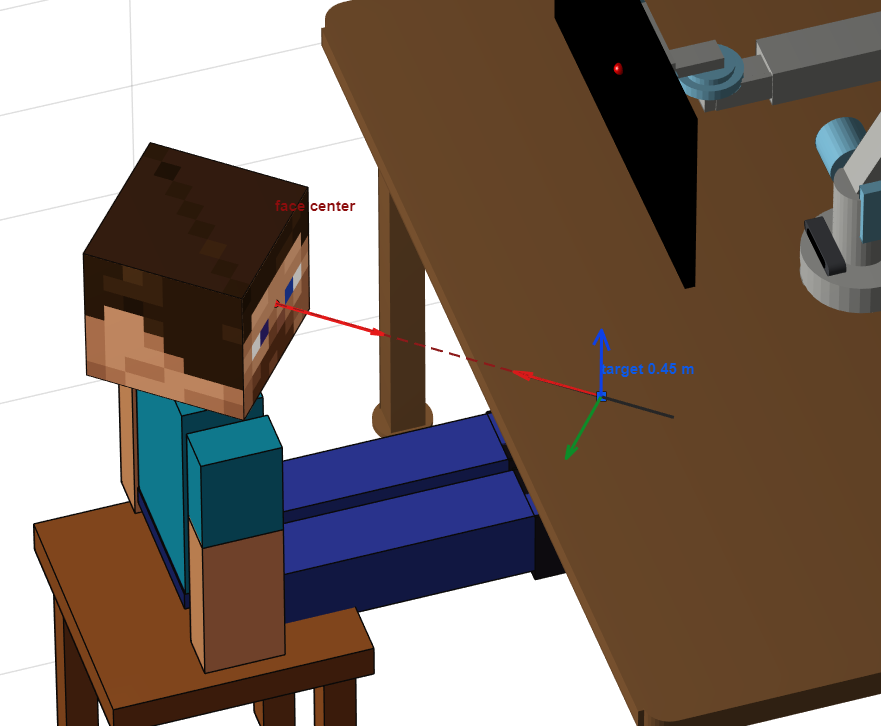
\includegraphics[width=0.66\textwidth]{目标位姿计算.png}
    \par\vspace{0.3em}
    {\small 由人脸方向向量来计算末端目标位姿}
\end{figure}

\begin{figure}[H]
    \centering
    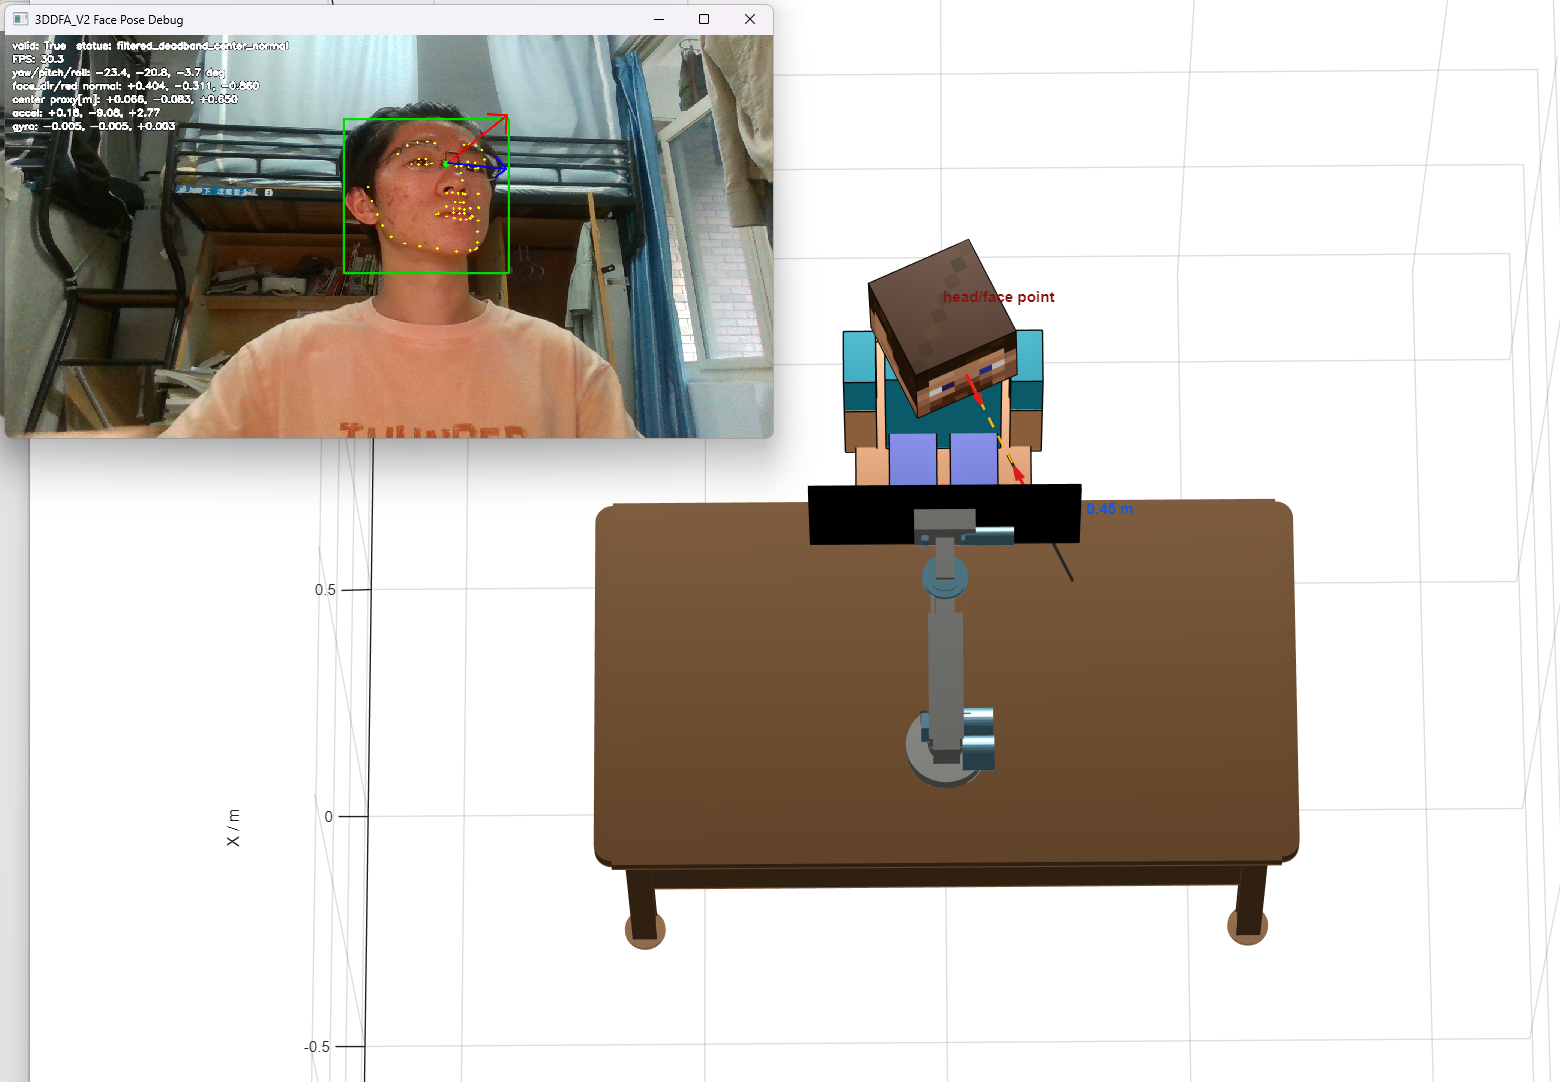
\includegraphics[width=0.66\textwidth]{人脸姿态到史蒂夫姿态的映射.png}
    \par\vspace{0.3em}
    {\small 人脸姿态到人偶姿态映射}
\end{figure}

\begin{figure}[H]
    \centering
    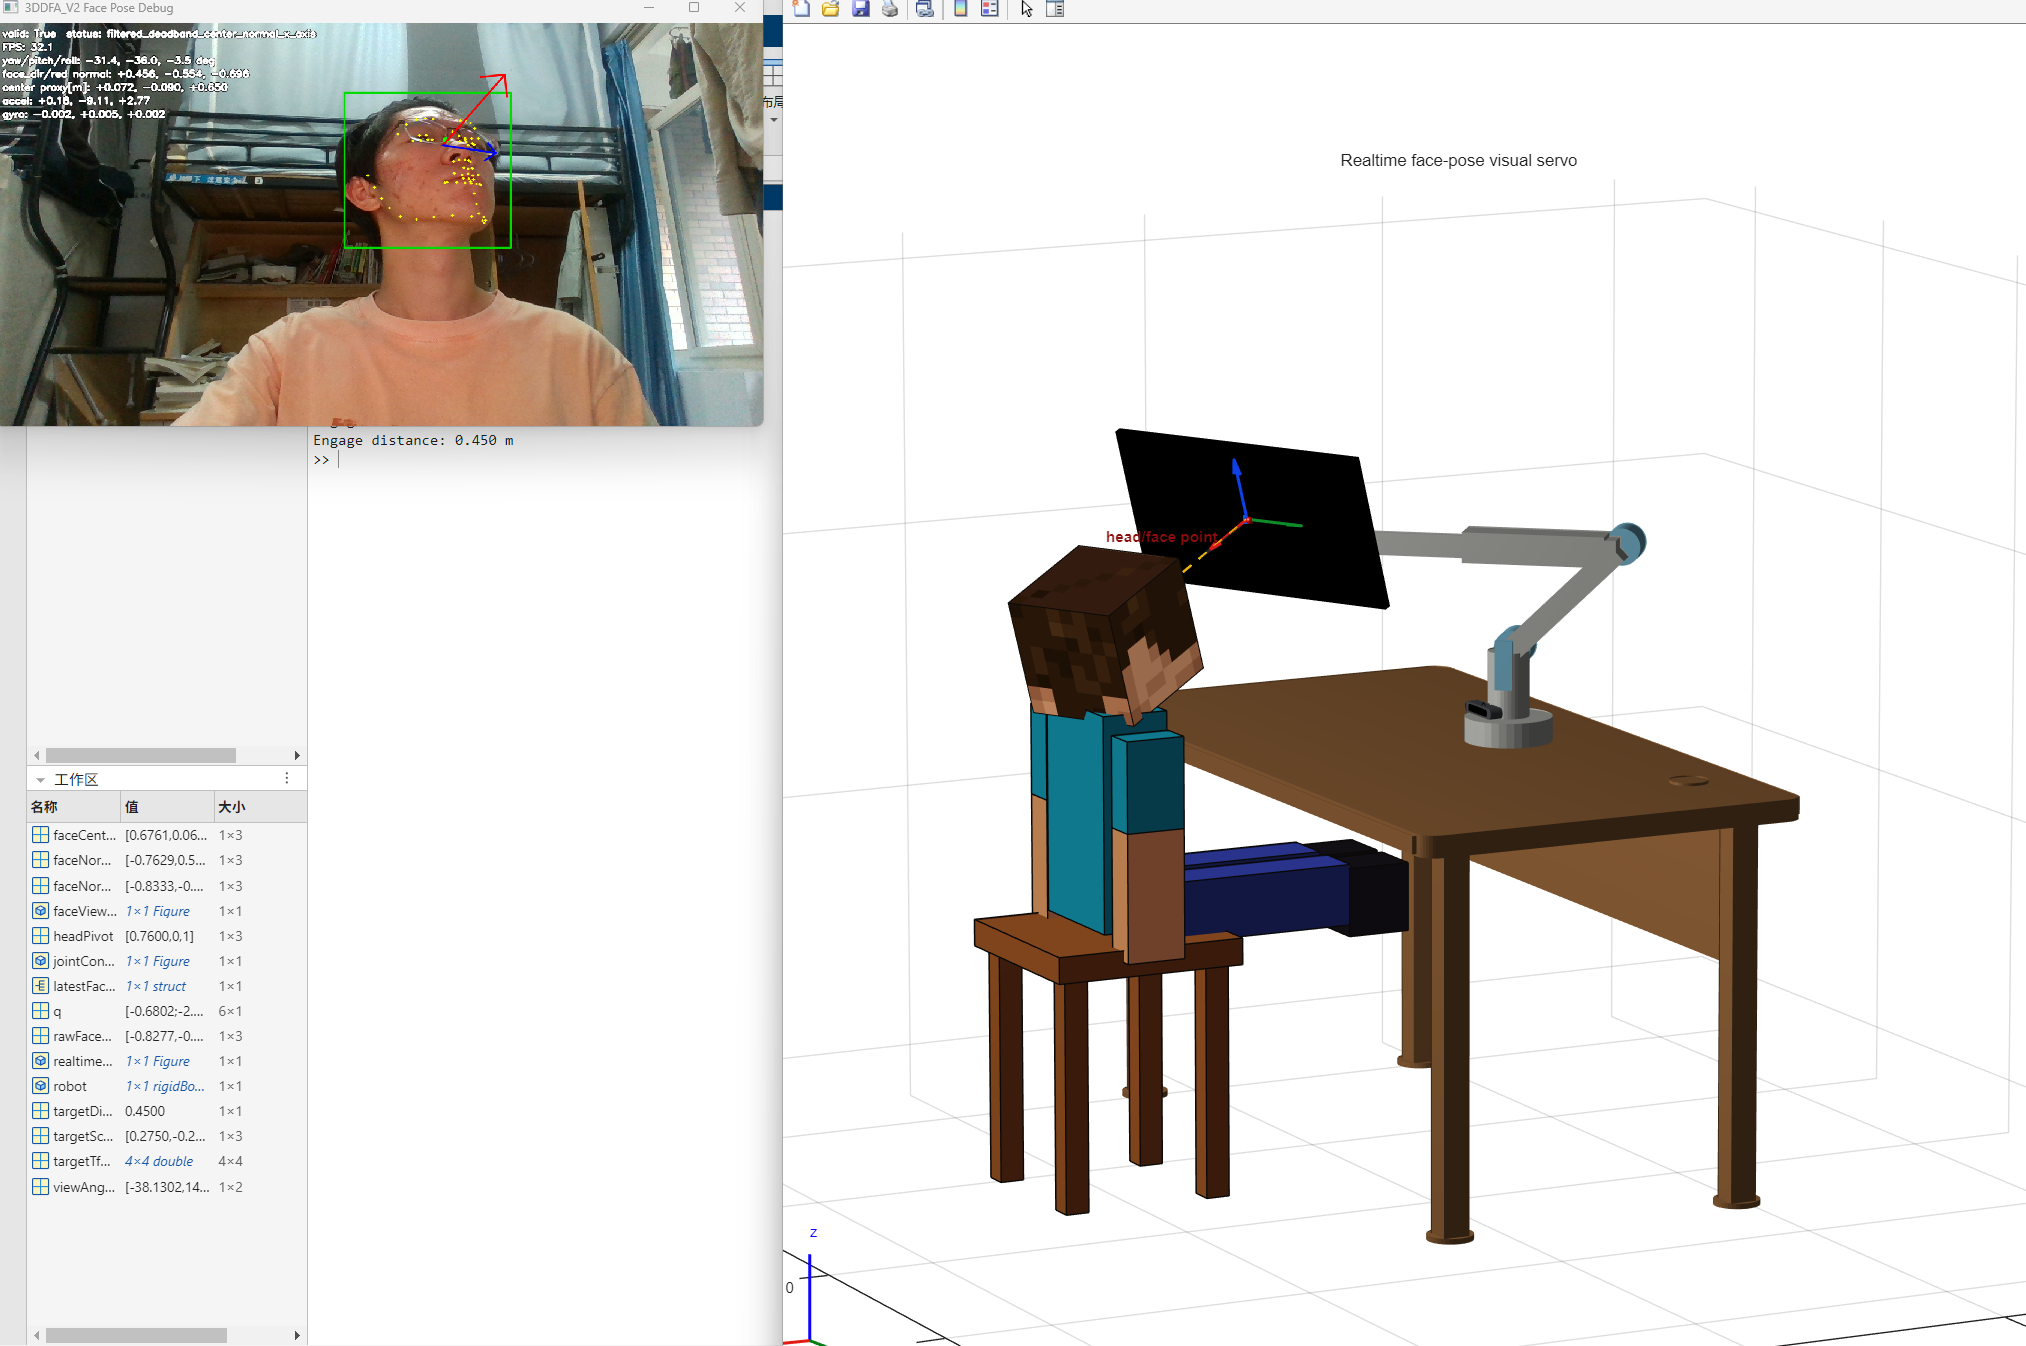
\includegraphics[width=0.66\textwidth]{屏幕跟随示意.png}
    \par\vspace{0.3em}
    {\small 屏幕跟随到合适位置}
\end{figure}

\subsection{逆运动学与距离容忍机制}

屏幕到人脸的距离并不需要严格固定在唯一值上。为了扩大机械臂可达范围，本项目将理想距离设为 $0.45\,\mathrm{m}$，同时允许屏幕中心到人脸中心的距离位于 $0.30\sim 0.60\,\mathrm{m}$ 范围内。控制程序首先尝试 $d=0.45\,\mathrm{m}$ 对应的目标位姿；若该目标不可达，则在允许距离范围内选取若干候选距离，依次构造目标位姿并进行逆运动学求解。

逆运动学求解的目标是寻找关节变量 $q$，使末端实际位姿 ${}^{W}_{S}T(q)$ 尽量接近目标位姿 ${}^{W}_{S}T^{*}$。在判断可达性时，程序主要检查三个条件：末端位置误差是否足够小、屏幕法向误差是否足够小、实际屏幕距离是否落在容忍区间内。若多个候选距离都可达，则优先选择更接近 $0.45\,\mathrm{m}$ 的结果。

具体求解时，程序调用 MATLAB Robotics System Toolbox 中基于 \texttt{rigidBodyTree} 的数值逆运动学求解器。该求解器并不直接推导解析闭式解，而是从当前关节变量 $q_0$ 出发，通过迭代优化寻找一组满足目标位姿的关节变量。可以将其理解为求解如下加权误差最小化问题：
\begin{equation}
    q^{*}
    =
    \arg\min_q
    \left(
        e(q)^{T}We(q)
    \right),
\end{equation}
其中 $e(q)$ 表示由末端实际位姿 ${}^{W}_{S}T(q)$ 和目标位姿 ${}^{W}_{S}T^{*}$ 之间的位置误差、姿态误差组成的误差向量，$W$ 为位置和姿态误差的权重矩阵。程序中使用当前关节状态作为初值，可以使求解结果尽量靠近机械臂当前姿态，从而减少不必要的大幅关节跳变。同时，求解过程会受到各关节运动范围的约束，避免得到超出机械结构限制的关节变量。

\subsection{离散式目标跟随方案}

在第三版测试程序中，机械臂采用离散式目标跟随策略。人脸姿态预览会持续刷新，但机械臂不会对每一帧微小变化都立即运动；只有当目标点位置变化或人脸法向量变化超过设定阈值时，程序才重新计算目标位姿并执行一次逆运动学求解。求得目标关节变量后，关节从当前状态平滑插值到目标状态。

设一次规划开始时的关节变量为 $q_0$，逆运动学求得的目标关节变量为 $q^{*}$，轨迹总时间为 $T$。为了使运动开始和结束时的速度为零，程序采用三次平滑插值因子
\begin{equation}
    s(t)=3\left(\frac{t}{T}\right)^2
    -2\left(\frac{t}{T}\right)^3,
    \qquad 0\leq t\leq T .
\end{equation}
于是关节轨迹可以写为
\begin{equation}
    q(t)=q_0+s(t)(q^{*}-q_0).
\end{equation}
该插值方式满足 $s(0)=0$、$s(T)=1$，并且在起点和终点处速度为零，因此比简单线性插值更平滑。实际程序中，轨迹点数会根据本次运动的最大关节变化量自动调整：关节变化越大，插值帧数越多；关节变化较小时，则使用较少帧数，以提高跟随响应速度。

该方案的优点是稳定、易于观察，也便于判断哪些目标姿态可达；缺点是跟随动作呈现为一段一段的运动。当用户头部连续转动时，机械臂需要等待一次规划完成后才能执行下一次规划，因此实时性有限。第三版方案主要用于验证目标位姿生成、距离容忍和不可达诊断逻辑。

\subsection{连续实时伺服方案}

第四版测试程序在离散式方案的基础上加入了连续实时伺服控制。点击开始跟随后，系统首先通过逆运动学和轨迹插值完成一次粗到位，使机械臂进入目标附近；随后进入连续伺服模式。在伺服模式中，程序每个控制周期都会根据最新人脸法向量更新目标位姿，并计算当前末端位姿与目标位姿之间的位置误差和姿态误差。

设末端速度旋量为 $V_S$，机械臂末端雅可比矩阵为 $J_S(q)$，则有
\begin{equation}
    V_S=J_S(q)\dot{q}.
\end{equation}
控制程序根据位置误差和姿态误差构造期望末端速度 $V_S^{*}$，再由阻尼最小二乘方法求关节速度：
\begin{equation}
    \dot{q}
    =
    J_S^T(q)
    \left(
        J_S(q)J_S^T(q)+\lambda^2 I
    \right)^{-1}
    V_S^{*}.
\end{equation}
其中 $\lambda$ 为阻尼系数。当机械臂接近奇异位形时，适当增大 $\lambda$ 可以抑制关节速度突增，提高跟随过程的稳定性。得到关节速度后，控制器按控制周期 $\Delta t$ 进行积分：
\begin{equation}
    q_{k+1}=q_k+\dot{q}_k\Delta t .
\end{equation}

这种方法不再等待完整轨迹规划结束，而是持续根据当前误差进行小步调整，因此比离散式目标跟随更接近实时控制效果。

\subsection{滤波、防抖与安全保护}

由于人脸姿态估计存在一定噪声，如果直接使用原始法向量控制机械臂，屏幕会出现明显抖动。为此程序对人脸法向量进行了滤波处理：当新法向量与上一帧法向量夹角很小时，认为该变化属于轻微抖动，不立即更新目标方向；当夹角较大时，采用球面插值逐步更新方向，并限制单位时间内允许变化的最大角度。相机 IMU 估计得到的俯仰角也经过低通滤波后再参与坐标变换。

在关节层面，控制程序对每个关节设置速度上限，并在更新关节变量后再次检查关节限位。若某一步计算得到的关节速度超过上限，则按比例缩放所有关节速度，保证运动不会过快。若实时伺服过程中连续多帧出现误差不收敛且关节速度接近饱和，程序会触发一次恢复机制，重新通过逆运动学进行粗到位。上述处理可以降低人脸姿态噪声、奇异位形和关节限位对系统稳定性的影响。

\clearpage
\section{仿真验证}

\subsection{实验环境}

本项目采用 Intel RealSense D435i 深度相机采集用户人脸图像和相机姿态信息。实验时，相机放置在桌面前方并朝向用户面部，用于实时估计用户人脸姿态；机械臂和屏幕的运动过程则在 MATLAB 仿真环境中展示。仿真环境中包含桌面、机械臂、屏幕、深度相机示意模型以及人偶模型，可以较直观地观察人脸姿态变化、屏幕目标位姿计算和机械臂跟随运动之间的关系。

\subsection{数据传输方式}

人脸姿态估计模块输出的人脸方向向量和相机俯仰角信息通过 UDP 方式传输到 MATLAB 仿真端。MATLAB 端接收到数据后，先将人脸方向从相机坐标系转换到世界坐标系，再结合固定的人头中心位置和期望观看距离计算屏幕目标位姿。随后，控制系统根据目标位姿进行逆运动学求解和轨迹生成，使机械臂末端屏幕逐步运动到合适位置。采用 UDP 传输可以减少文件读写带来的延迟，更适合人脸姿态连续变化时的实时跟随验证。

\subsection{逆运动学、轨迹规划功能验证}

为了单独验证逆运动学和轨迹规划模块，实验中先在仿真界面中人为设定一个目标人脸朝向，再由程序计算对应的屏幕目标位姿，并求解机械臂从初始姿态运动到目标姿态所需的关节变量。图中设置的人脸方向为偏摆角 $34.5^\circ$、俯仰角 $21.4^\circ$，目标观看距离为 $0.45\,\mathrm{m}$。根据该目标方向计算得到的屏幕中心目标点为
\begin{equation}
    p_s^{*}
    =
    \begin{bmatrix}
        0.330273 & -0.295129 & 1.204532
    \end{bmatrix}^{T}\mathrm{m}.
\end{equation}

\begin{figure}[H]
    \centering
    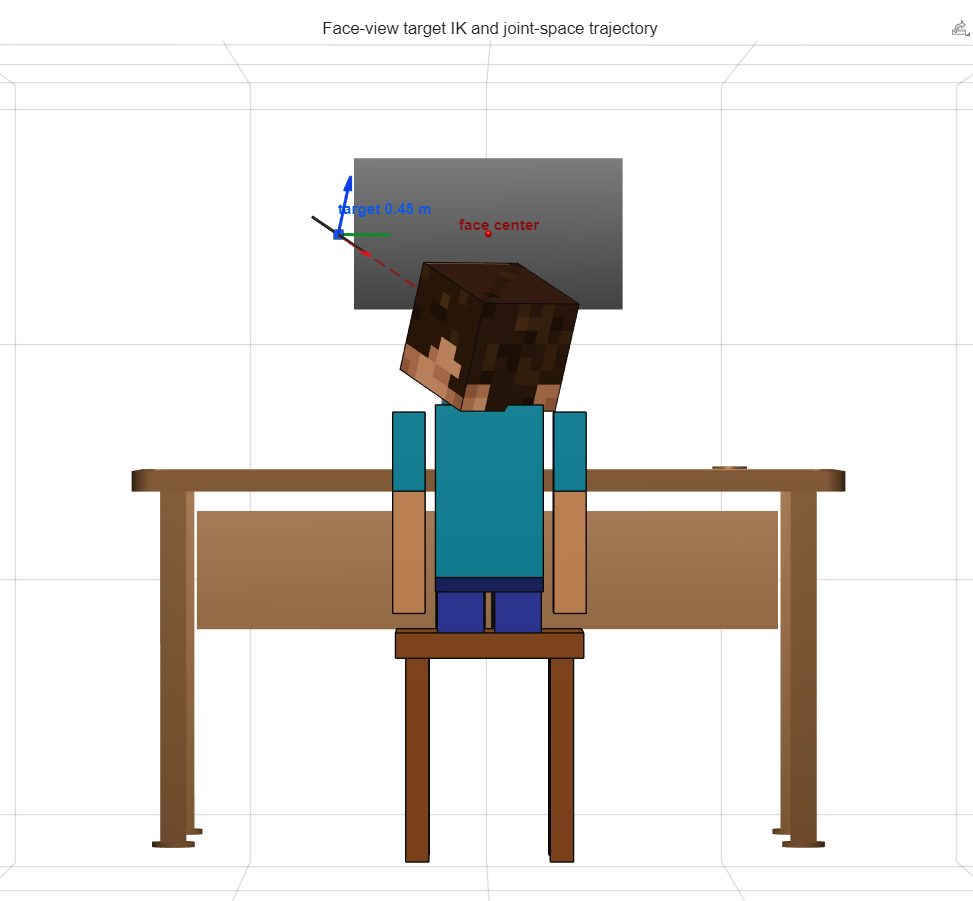
\includegraphics[width=0.72\textwidth]{设定一个目标点来算轨迹.png}
    \par\vspace{0.3em}
    {\small 设定目标点并计算轨迹}
\end{figure}

逆运动学求解结果表明，该目标位姿在机械臂工作空间内可达，末端位置误差为 $1.07\times 10^{-8}\,\mathrm{m}$，屏幕法向误差近似为 $0^\circ$。求解得到的目标关节变量为
\begin{equation}
    q^{*}
    =
    \begin{bmatrix}
        -43.423^\circ & -66.887^\circ & 66.887^\circ & 91.959\,\mathrm{mm} & 77.904^\circ & 21.422^\circ
    \end{bmatrix}^{T}.
\end{equation}
随后对各关节变量采用平滑插值生成 $2\,\mathrm{s}$ 内的关节空间轨迹。六个关节的曲线均从初始值平滑过渡到目标值，起点和终点处变化速度较小，说明轨迹规划能够避免突变式运动，适合作为仿真中机械臂到达目标位姿的控制输入。

\begin{figure}[H]
    \centering
    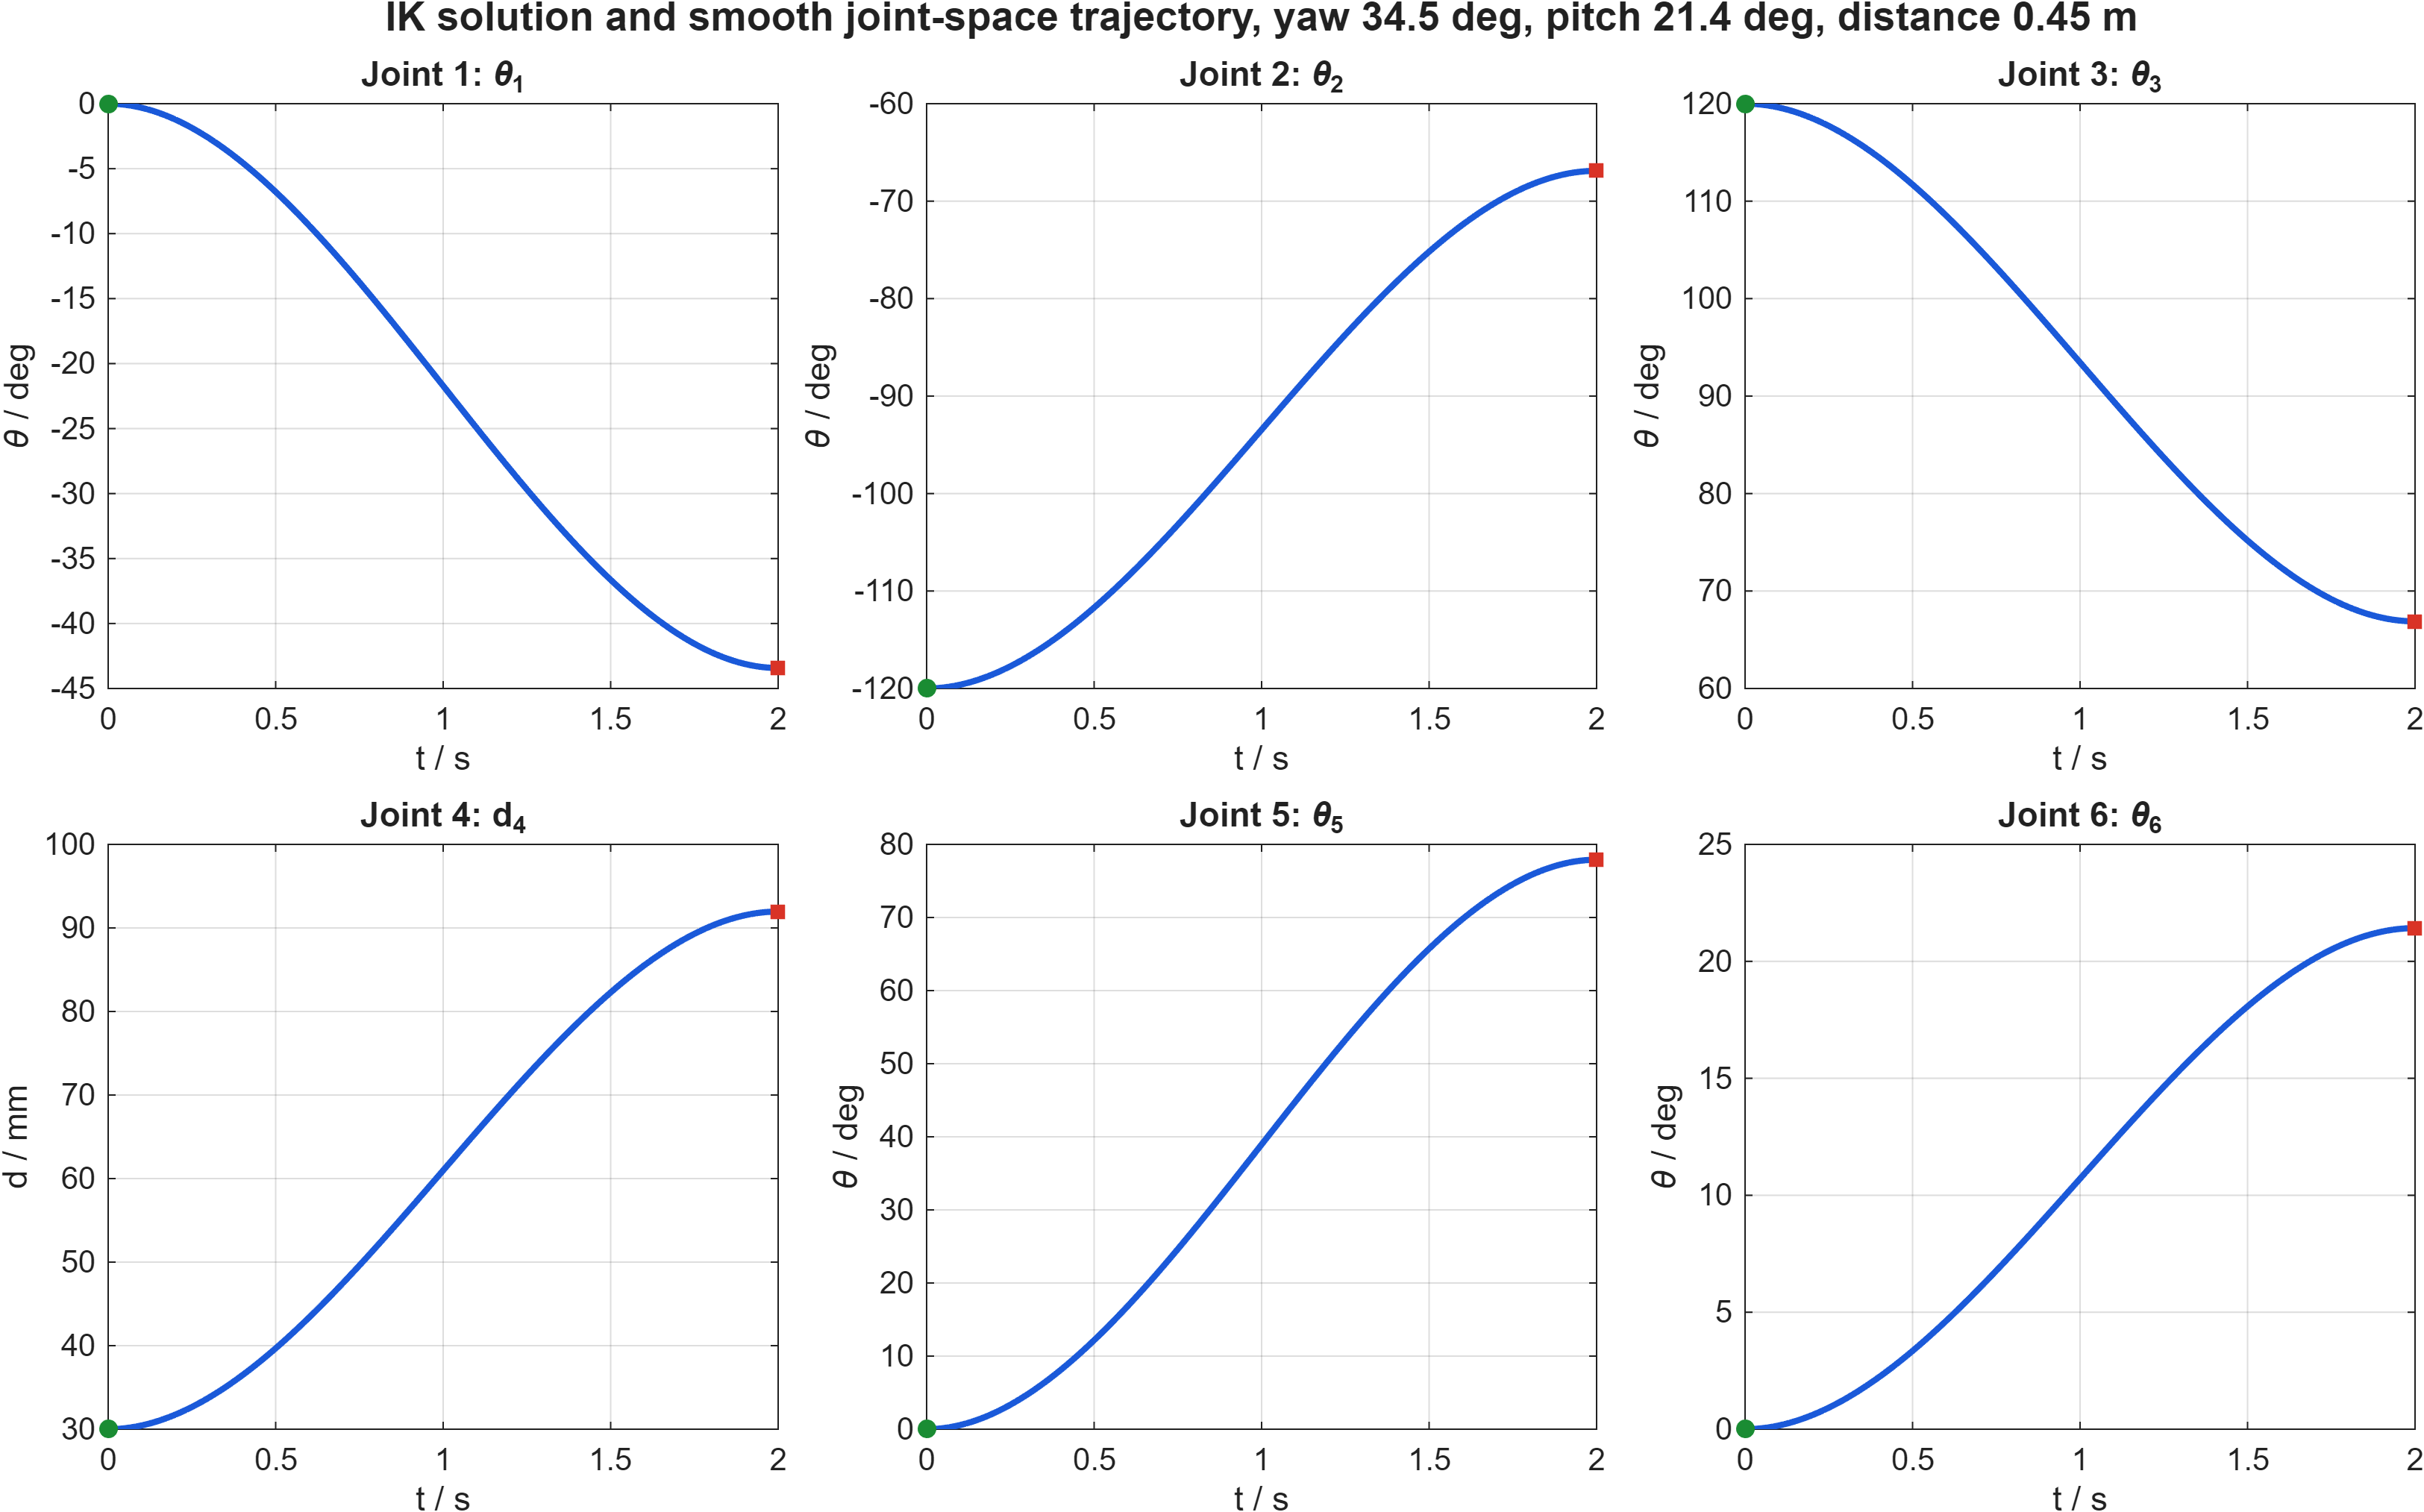
\includegraphics[width=\textwidth]{逆运动学关节轨迹曲线.png}
    \par\vspace{0.3em}
    {\small 六个关节的规划轨迹曲线}
\end{figure}

\subsection{验证结果}

实验结果表明，在较理想的工作空间范围内，系统能够实现稳定的屏幕随动效果。当用户人脸偏摆角位于 $-45^\circ$ 到 $+45^\circ$ 范围内时，机械臂能够较好地保持屏幕中心位于用户视线方向上，并使屏幕平面基本正对人脸。仿真过程中，人偶头部姿态、目标位姿箭头和机械臂运动状态能够同步变化，说明人脸姿态感知、坐标变换、目标位姿计算和机械臂运动控制之间的链路已经基本打通。项目最终拍摄了视频 demo，用于展示系统在连续人脸姿态变化下的跟随效果。

\clearpage
\section{优化与总结}

\subsection{可优化方向}

本项目已经完成了从人脸姿态感知到机械臂屏幕跟随的完整仿真验证，但仍然存在一些可以继续优化的方向。

首先，当前控制系统中采用了“人头中心点固定”的简化假设，即认为用户只改变人脸姿态，而人脸中心位置不发生变化。该假设有利于降低前期建模和控制难度，但与真实使用场景仍有差距。实际使用中，用户的头部一定会发生小范围平移，例如身体前倾、后靠或左右移动。因此，后续可以进一步引入人脸中心位置估计，使系统同时跟踪人脸位置和人脸姿态，从而更接近真实使用需求。

其次，当前机械臂结构仍然不能覆盖全部极限姿态需求。当人脸偏摆角超出约 $45^\circ$ 范围后，部分目标位姿会接近或超出机械臂工作空间，导致逆运动学求解失败或关节接近限位。同时，本项目中的机械臂结构仍然较为简单，整体上以前四个关节主要负责末端位置调整、后两个关节主要负责末端姿态调整。对于屏幕随动这一特定任务，结构上可能还存在更优方案，例如增加自由度、调整关节布置位置、优化伸缩关节行程，或重新设计末端腕部结构。

第三，目前人脸姿态建模主要采用端到端姿态估计方式。该方法实现较方便，实时性较好，但对光照、遮挡和人脸检测稳定性仍较敏感。后续可以进一步利用高精度深度相机返回的三维点云信息，对人脸区域进行更精确的三维建模，例如直接拟合人脸局部平面或构建面部关键点三维模型，以提高人脸姿态估计的精度和稳定性。

最后，当前测试主要在 MATLAB 仿真环境中完成，尚未引入真实物理环境和完整物理引擎。因此，仿真结果还不能完全代表真实使用情况。若后续进行实物开发，需要进一步推敲机械结构强度、关节间隙、屏幕重量、线缆布置、电机选型、减速器选型和控制安全性等问题，尤其要验证屏幕在实际运动过程中的稳定性和安全边界。

\subsection{项目总结}

本项目围绕“基于人脸姿态感知的机器人电脑屏幕随动系统”这一目标，完成了人脸姿态估计、坐标变换、目标位姿生成、逆运动学求解、轨迹规划和实时仿真验证等主要工作。系统能够利用深度相机获取用户人脸姿态信息，并在仿真环境中驱动机械臂调整屏幕位置和朝向，使屏幕尽量保持在用户视线方向上并正对人脸。

从课程设计角度看，本项目将机器人学中的运动学建模、逆运动学、轨迹规划、工作空间分析和驱动选型等知识串联到了一个较完整的应用场景中。通过多轮测试和迭代，项目从单独的机械臂模型演示逐步扩展到人脸姿态感知与机械臂控制联合仿真，最终实现了较稳定的屏幕随动效果。虽然当前系统仍处于仿真验证阶段，但已经验证了方案的基本可行性，也为后续实物样机开发提供了较清晰的技术路线。

本项目已开源在 GitHub 上，欢迎来点星星，项目链接为：
\begin{center}
    \url{https://github.com/Hippo1013/screen_arm}
\end{center}

\clearpage

% \appendix

% \section{附录1：}

% \begin{lstlisting}
% \end{lstlisting}


% \section{附录2：}
% \reference






\end{document}
